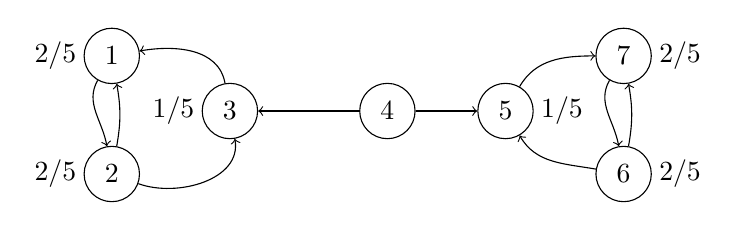
\begin{tikzpicture}
\tikzstyle{every node}=[draw,circle,fill=white,minimum size=20pt,
inner sep=0pt]

\draw (-1.5,0)  node (1) [label=left:$2/5$] {1};
\draw (-1.5 ,-1.5)  node (2) [label=left:$2/5$] {2};
\draw (0,-0.7)  node (3) [label=left:$1/5$] {3};
\draw [->] (1) to  [out = 240, in = 100] (2);
\draw [->] (2)to  [out = 80, in = 280](1);
\draw [->] (3)to  [out = 100, in = 10](1);
\draw [->] (2)to  [out = 340, in = 280](3);
\draw (2,-0.7)  node (4) [label=left:$$] {4};
\draw [->] (4)to  [out = 180, in = 0](3);
\draw (3.5,-0.7)  node (5) [label=right:$1/5$] {5};
\draw [->] (4)to  [out = 0, in = 180](5);
\draw (5,0)  node (7) [label=right:$2/5$] {7};
\draw (5 ,-1.5)  node (6) [label=right:$2/5$] {6};

\draw [->] (7) to  [out = 240, in = 100] (6);
\draw [->] (6)to  [out = 80, in = 280](7);
\draw [->] (5)to  [out = 60, in = 180](7);
\draw [->] (6)to  [out = 170, in = 300](5);
\end{tikzpicture}